\section{Límites y Continuidad de funciones}

Consideremos la función $f : \R \to \R$, $x \mapsto f(x) = \dfrac{x^3 -1}{x-1}$. Observemos que $f$ no está definida en $x=1$, ya que el denominador se anula. Sin embargo, surge una pregunta fundamental: \textbf{¿podemos decir algo sobre el comportamiento de la función $f$ cerca del punto $x=1$?}. Exploraremos esta idea calculando algunos valores de $f$ para $x$ cercanos a $1$:

\begin{center}
\begin{minipage}{0.45\textwidth}
    \centering
    \renewcommand{\arraystretch}{1.5}
    \begin{tabular}{|c|c|}
        \hline
        $x$ & $f(x) = \frac{x^3 - 1}{x - 1}$ \\
        \hline
        0.9   & 2.710000 \\
        0.99  & 2.970100 \\
        0.999 & 2.997001 \\
        \hline
        1 &  Indefinido \\
        \hline
        1.001 & 3.003001 \\
        1.01  & 3.030100 \\
        1.1   & 3.310000 \\
        \hline
    \end{tabular}
\end{minipage}%
\hfill
\begin{minipage}{0.5\textwidth}
    \centering
    \begin{tikzpicture}
        \begin{axis}[
            axis lines = center,
            xlabel = {$x$},
            ylabel = {$f(x)$},
            xmin = -2.5, xmax = 3.5,
            ymin = -1, ymax = 15,
            ytick = {3,5,7,9,11,13},
            domain = -2:3,
            samples = 100,
            width = \textwidth,
            grid = major,
            grid style = {dashed, gray!30},
            every axis x label/.style={at={(ticklabel* cs:1.05)},anchor=west},
            every axis y label/.style={at={(ticklabel* cs:1.05)},anchor=south},
        ]
        
        % Dibujamos la función simplificada x^2 + x + 1
        \addplot [blue, thick] {x^2 + x + 1};
        
        % Añadimos el punto vacío en x=1, y=3
        \addplot[mark=*, mark options={fill=white, draw=blue, thick}, only marks] coordinates {(1,3)} node[anchor=north west, text=black] {};

        % Líneas discontinuas hacia los ejes
        \draw [dashed, gray, thick] (axis cs:1,0) -- (axis cs:1,3);
        \draw [dashed, gray, thick] (axis cs:0,3) -- (axis cs:1,3);
        
        \end{axis}
    \end{tikzpicture}
\end{minipage}
\end{center}

Al analizar tanto numéricamente como gráficamente, observamos que a medida que $x$ se aproxima a $1$, los valores de $f(x)$ se acercan a $3$. Esto nos lleva a la conclusión de que, aunque $f$ no está definida en $x=1$, podemos afirmar que cuando los valores de $x$ se acercan a $1$, los valores de $f(x)$ se acercan a $3$. En notación matemática, esto se expresa como:
\[ \lim_{x \to 1}{f(x)} = \lim_{x \to 1}{\frac{x^3 -1}{x-1}} = 3 = L. \]
Esto significa que que podemos hacer que $f(x)$ esté \textbf{tan cerca de $3$ como queramos}, siempre y cuando el valor de $x$ esté lo suficientemente cerca (aunque no exactamente) de $1$.

\textbf{¿Qué significa exactamente que $f(x)$ esté cerca de $L$?}. En matemática, \textbf{medir} la cercanía de dos números se hace a través de la \textbf{distancia} entre ellos, que se define como el \textbf{valor absoluto de su diferencia}.

\begin{center}
\begin{minipage}{0.45\textwidth}
    Decir que $f(x)$ está cerca de $L$ significa que la distancia entre $f(x)$ y $L$ es pequeña, es decir, que $|f(x) - L| < \varepsilon$, donde $\varepsilon > 0$ representa una tolerancia o margen de error. Esto significa que los valores de $f(x)$ pertenecen al intervalo $]L - \varepsilon, L + \varepsilon[$.
\end{minipage}%
\hfill
\begin{minipage}{0.45\textwidth}
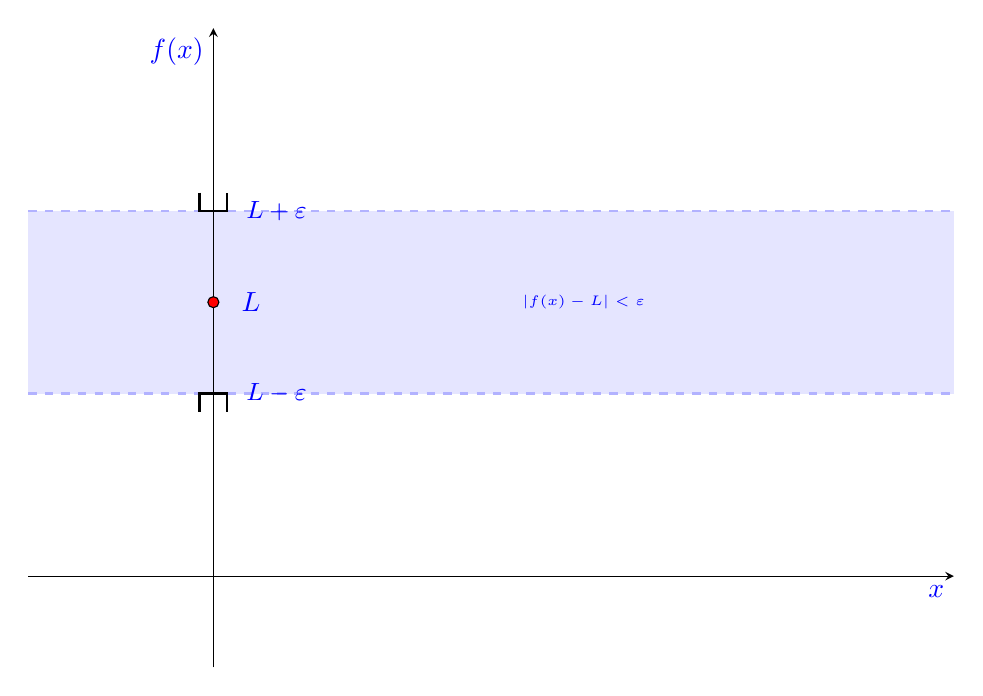
\begin{tikzpicture}
    \begin{axis}[
        axis lines = center,
        xlabel = {\color{blue}$x$},
        ylabel = {\color{blue}$f(x)$},
        xmin = -2, xmax = 8,
        ymin = -1, ymax = 6,
        xtick = \empty,
        ytick = \empty,
        % MODIFICACIÓN: Aumentamos el tamaño general de la gráfica
        width = 1.1\textwidth,
        height = 0.8\textwidth,
        every axis x label/.style={at={(ticklabel* cs:1.0)},anchor=north east},
        every axis y label/.style={at={(ticklabel* cs:1.0)},anchor=north east},
        axis on top, 
    ]
    
    % 1. Franja horizontal (Banda del intervalo)
    \fill[blue!10] (axis cs:-2, 2) rectangle (axis cs:8, 4);
    
    % Bordes punteados suaves para delimitar la franja
    \draw[blue!30, dashed, thick] (axis cs:-2, 4) -- (axis cs:8, 4);
    \draw[blue!30, dashed, thick] (axis cs:-2, 2) -- (axis cs:8, 2);

    % 2. Texto central de la inecuación (tamaño aumentado a \LARGE)
    \node[text=blue, font=\tiny] at (axis cs: 4, 3) {$|f(x) - L| < \varepsilon$};

    % 3. Marcador del punto L (Punto rojo en el eje Y)
    \addplot[mark=*, mark options={fill=red, draw=black}, only marks] coordinates {(0,3)};
    \node[blue, right] at (axis cs: 0.2, 3) {$L$};

    % 4. Corchete superior para L + \varepsilon
    % Ajustado a 0.15 para mantener la proporción visual al ensanchar la gráfica
    \draw[thick] (axis cs:-0.15, 4.2) -- (axis cs:-0.15, 4) -- (axis cs:0.15, 4) -- (axis cs:0.15, 4.2);
    \node[blue, right, font=\small] at (axis cs: 0.25, 4) {$L+\varepsilon$};

    % 5. Corchete inferior para L - \varepsilon
    \draw[thick] (axis cs:-0.15, 1.8) -- (axis cs:-0.15, 2) -- (axis cs:0.15, 2) -- (axis cs:0.15, 1.8);
    \node[blue, right, font=\small] at (axis cs: 0.25, 2) {$L-\varepsilon$};

    \end{axis}
\end{tikzpicture}
\end{minipage}
\end{center}

\begin{center}
\begin{minipage}{0.45\textwidth}
    Analógamente, decir que $x$ está cerca de $a$ significa que la distancia entre $x$ y $a$ es pequeña, es decir, que $|x - a| < \delta$, donde $\delta > 0$ representa una tolerancia o margen de error. Esto significa que los valores de $x$ pertenecen al intervalo $]a - \delta, a + \delta[$.
\end{minipage}%
\hfill
\begin{minipage}{0.45\textwidth}
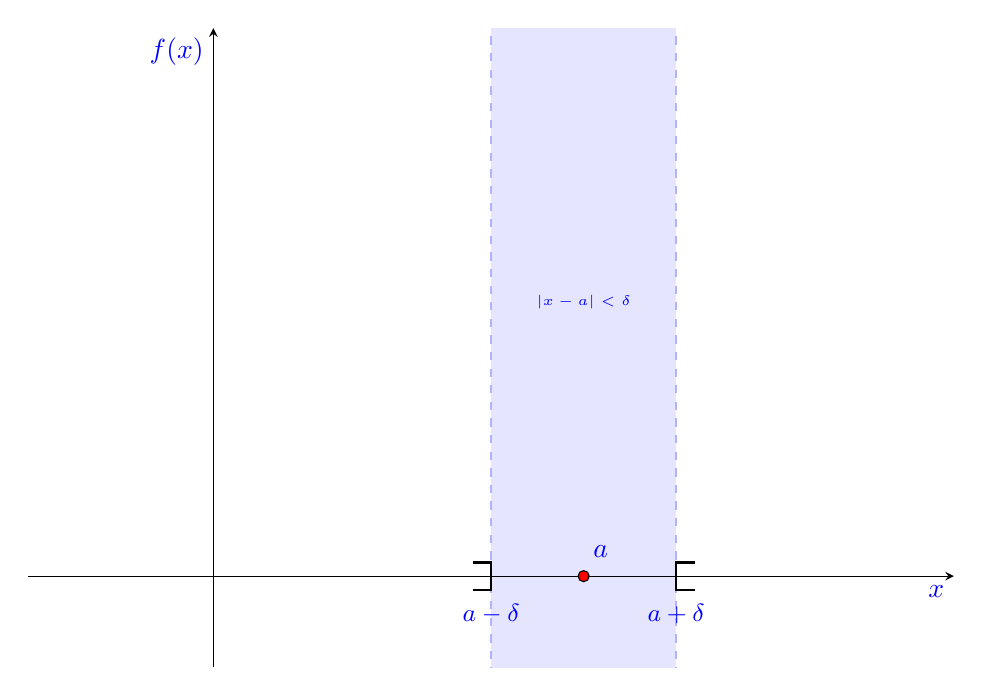
\begin{tikzpicture}
    \begin{axis}[
        axis lines = center,
        xlabel = {\color{blue}$x$},
        ylabel = {\color{blue}$f(x)$},
        % Ajustamos los límites para centrar la gráfica en el eje x
        xmin = -2, xmax = 8,
        ymin = -1, ymax = 6,
        xtick = \empty,
        ytick = \empty,
        width = 1.1\textwidth,
        height = 0.8\textwidth,
        every axis x label/.style={at={(ticklabel* cs:1.0)},anchor=north east},
        every axis y label/.style={at={(ticklabel* cs:1.0)},anchor=north east},
        axis on top, 
    ]
    
    % 1. Franja vertical (Banda del intervalo en el eje x)
    \fill[blue!10] (axis cs:3, -2) rectangle (axis cs:5, 6);
    
    % Bordes punteados suaves para delimitar la franja verticalmente
    \draw[blue!30, dashed, thick] (axis cs:3, -2) -- (axis cs:3, 6);
    \draw[blue!30, dashed, thick] (axis cs:5, -2) -- (axis cs:5, 6);

    % 2. Texto central de la inecuación (ajustado a un tamaño legible)
    \node[text=blue, font=\tiny] at (axis cs: 4, 3) {$|x - a| < \delta$};

    % 3. Marcador del punto 'a' (Punto rojo en el eje X)
    \addplot[mark=*, mark options={fill=red, draw=black}, only marks] coordinates {(4,0)};
    \node[blue, above right] at (axis cs: 4, 0.1) {$a$};

    % 4. Corchete derecho para a + \delta en el eje X
    \draw[thick] (axis cs:5.2, -0.15) -- (axis cs:5, -0.15) -- (axis cs:5, 0.15) -- (axis cs:5.2, 0.15);
    \node[blue, below, font=\small] at (axis cs: 5, -0.2) {$a+\delta$};

    % 5. Corchete izquierdo para a - \delta en el eje X
    \draw[thick] (axis cs:2.8, -0.15) -- (axis cs:3, -0.15) -- (axis cs:3, 0.15) -- (axis cs:2.8, 0.15);
    \node[blue, below, font=\small] at (axis cs: 3, -0.2) {$a-\delta$};

    \end{axis}
\end{tikzpicture}
\end{minipage}
\end{center}


\begin{definition}{Límites}{def:limite}
    Se dice que el límite de una función $f(x)$ cuando $x$ tiende a un valor $a$ es igual a un número $L$, y se denota como
    \[
        \lim_{x \to a} f(x) = L,
    \]
    si para todo $\epsilon > 0$ existe un $\delta > 0$ tal que si $0 < |x - a| < \delta$, entonces $|f(x) - L| < \epsilon$.
\end{definition}

\subsection{Límites laterales}

\begin{center}
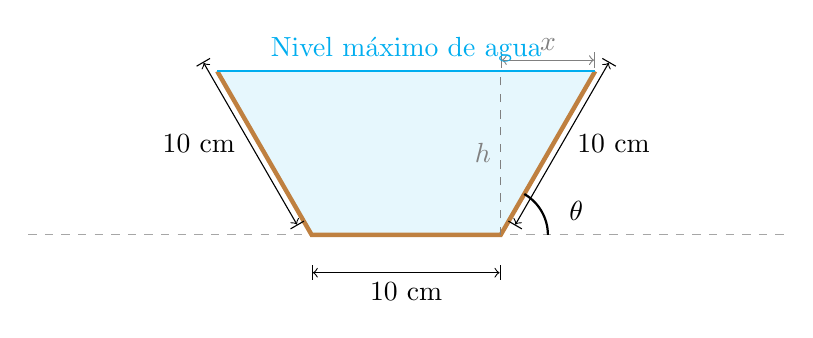
\begin{tikzpicture}[scale=1.2]
    % Eje horizontal base punteado
    \draw[dashed, gray!70] (-3,0) -- (5,0);
    
    % Relleno del agua (Trapecio)
    \fill[cyan!10] (0,0) -- (2,0) -- (3, 1.732) -- (-1, 1.732) -- cycle;
    
    % Plancha de acero corten (Perfil de la canaleta)
    \draw[ultra thick, brown] (-1, 1.732) -- (0,0) -- (2,0) -- (3, 1.732);
    
    % Cotas de la plancha (10 cm cada tercio)
    \draw[|<->|] (0, -0.4) -- (2, -0.4) node[midway, below] {10 cm};
    \draw[|<->|] (2.15, 0.1) -- (3.15, 1.832) node[midway, right, xshift=2pt] {10 cm};
    \draw[|<->|] (-0.15, 0.1) -- (-1.15, 1.832) node[midway, left, xshift=-2pt] {10 cm};
    
    % Ángulo theta
    \draw[thick] (2.5, 0) arc (0:60:0.5);
    \node at (2.8, 0.25) {$\theta$};
    
    % Proyecciones trigonométricas
    \draw[dashed, gray] (2, 1.732) -- (3, 1.732);
    \draw[dashed, gray] (2,0) -- (2, 1.732) node[midway, left] {$h$};
    \draw[|<->|, gray] (2, 1.85) -- (3, 1.85) node[midway, above] {$x$};
    
    % Nivel del agua
    \draw[cyan, thick] (-1, 1.732) -- (3, 1.732);
    \node[cyan, above] at (1, 1.732) {Nivel máximo de agua};

\end{tikzpicture}
\end{center}

\subsection{Límites infinitos y al infinito}

\subsection{Asíntotas}

\subsection{Continuidad de funciones}